Although continual learning is a general modeling concept, applicable in statistical inference as well as pattern driven prediction algorithms, it is mostly used in a machine learning context, more specifically in artificial neural networks (ANN). They are algorithms based on the functionality of a human brain and often designed for scenarios where data is seen in real-time, e.g. stock market predictions or power control systems. \citeauthor{Du_2019} \cite{Du_2019} and \citeauthor{Fahrmeir_2022} \cite{Fahrmeir_2022} provide an overview to this topic, which builds the foundation of this thesis. 

The simplest form of an ANN is a single linear classifier, called one-neuron perceptron, that devides a vector $x$ into two classes using a so-called activation function $h(\cdot)$. The neuron's input is given by
\begin{equation}
	\sum_{i = 1}^{n}{w_i x_i}+c = w^\top x+c
\end{equation}
where $n$ is the number of observations, $w$ a weight vector assigned to $x$ and $c$ the decision threshold. The two class regions are separated by the hyperplane%% \cite{Du_2019}
\begin{equation}
	w^\top x + c = 0
\end{equation}.
Using multiple neurons with the same activation function creates a one-layer perceptron and enables classification for more than two classes with the input
\begin{equation}
	\sum_{k = 1}^{m}\sum_{i=1}^{n}w_{k,i}x_i + c = (w_1^\top x + c, ..., w_m^\top x + c)^\top = W^\top x + c
\end{equation} 
, where $W$ is the $n\times m$ weight matrix and $m$ the number of classes. Given $h$ as the logistic function, a one-layer perceptron is equal to a multinomial logit model%%\cite{Fahrmeir_2022}
. Composing $l$ layers of neurons, Feed Forward NN (FFNN), allows for a more abstract representation of the data and finer class boundaries. Commonly, these layers are referred to as hidden layers, since only the input and output are observable. The unknown weight matrices $W_1, ..., W_l$ and the decision threshold $c$ are obtained by minimizing the empirical Risk of the network
\begin{equation}
	\mathcal{R}(f) = \sum_{i=1}^{n} L(f(x_i, \theta), y_i)
\end{equation}
, where $\theta$ are the unknown parameters and $L(\cdot)$ a loss function, which measures the discrepancy between the predicted values $\hat{y}_i = f(x_i, \theta)$ and the true values $y_i$. Risk minimization usually makes use of gradient-decent methods. They are numerical algorithms that converge to a local minimum in $\varepsilon$-neighborhood of the solution of parameters.
\begin{figure}[h!]
	\centering
	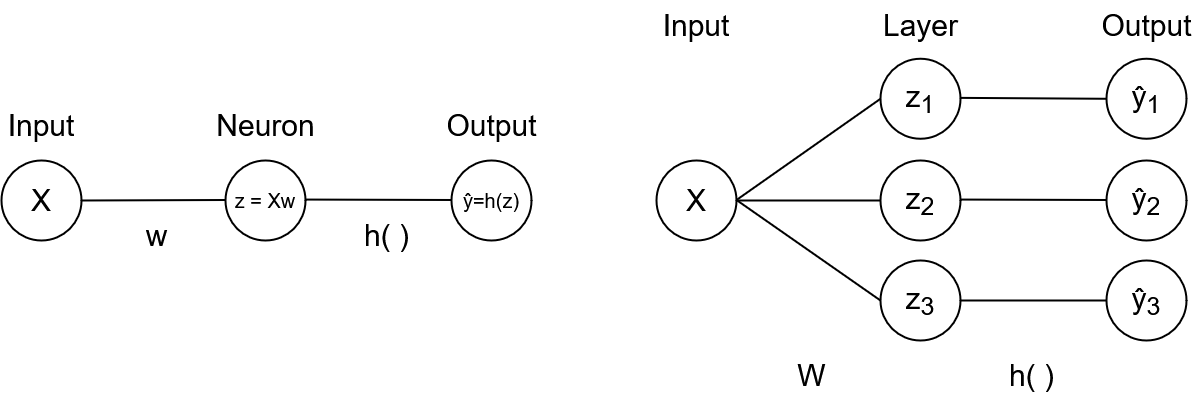
\includegraphics[width=0.9\textwidth]{img/perceptrons.png}
	\caption{A one-neuron perceptron (left) and a one-layer perceptron with 3 neurons (right).}
	\label{fig:P}
\end{figure}

In the following, modeling of a probability distribution over a data sample and learning how to predict the next output for an unseen data point will both be referred to as a \textit{task}. Both ideas are closely related, because inferred statistical models can be used to deduce long term behavior or to make a best guess about unobserved data.
